 
This work was first discussed as a possibility in  \citep{Schneider2014}  and 
forms the basis of the analyses performed in Schneider et al. (in prep.).

\section{Introduction} 
Conventional approach to infer cosmological parameters from lensed galaxies
from sky surveys is to use the 
two-point correlation function (2PCF), or aperture-mass dispersion.
% state what is a 2PCF 


Manual PSF tweaking 


We propose a flexible, generative regression model    
that can specify the joint distribution of the input variables while 
simultaneously capturing the rich physical relationships between the different
lensing observables.  

In this work, we 
1) illustrate the basic properties of the Gaussian Process and how it is
similar or different from other approaches for cosmic shear inference  \\ 
2) show the derivation for incorporating the lensing physics in 
a suitable covariance kernel form for a Gaussian Process  \\
3) lay out the statistical model for making several mass maps 
with the Gaussian Process with the modified kernel and show preliminary results \\ 
4) discuss possible extensions and future directions 
 
Our method provides an alternative from having to use the 2PCF to represent the
Gaussian perturbations and other higher order
statistics for representing the non-Gaussian part of the cosmic shear information. 
Source galaxies provide sparse constraints to probe the matter density along
the line of sight. 

\section{Method}
\subsection{The basics of a Gaussian Process}
A Gaussian Process is one of the most highly published and studied 
generative model. It allows the inference of the joint probability density 
function (PDF) for describing a set of data. The joint PDF can carry more information,
such as the uncertainties from the inputs, 
than summary statistics such as the two-point correlation function.
This gives the model the flexibility for a wide range
of successful applications in many fields. 
In Astronomy, a GP has been used for modeling 
the light curve of exoplanets \citep{Ambikasaran2014a}.
Or the GP can be used as a prior probability 
for optimizing the model parameters of
neural networks \citep{Snoek2012}, 
It has also been used for other classification and pattern extraction tasks 
(\citealt{Wilson2013}, \citealt{Duvenaud2013}, \citealt{Rasmussen2006}).
 
It is helpful to understand the mathematical formulation of a GP 
before discussing how we can adapt the GP to model the lensing observables. 
In a nutshell, a GP smooths the input data using a non-parametric kernel
\citep{Hastie1990}. 
It is the generalization of a multivariate Gaussian 
to infinite dimension \citep{Rasmussen2006}. 
While a multivariate Gaussian is parametrized by  
the mean vector $\mathbf{\mu}$ and the covariance matrix $\Sigma$, 
a GP is specified by a mean vector function $m(\xv)$ and a
covariance kernel function $\kerngp(\xv, \yv)$, based on some input spatial or
temporal coordinates $\xv$. In our case, the vector $\xv$ (and the
interchangeable notation $\yv$) denotes the
two-dimensional spatial coordinates of $\ngal$ source galaxy locations. 
The drawn collections of values $\psi(\xv)$ from a GP carry the correlation structures
specified by the kernel $\kerngp(\xv, \yv)$, and can be thought of as
functions: 
\begin{equation}
		[\psi_1(\xv), \psi_2(\xv) \ldots, \psi_m(\xv) ]^T \sim \gp(m(\xv), \kerngp(\xv, \xv')).
		\label{eq:GP}
\end{equation}
% Specifically, the mean vector $m(x)$ is often set to be zero in the
% GP. The data are usually mean-subtracted before fitting a GP.  
\begin{figure}
	\centering
	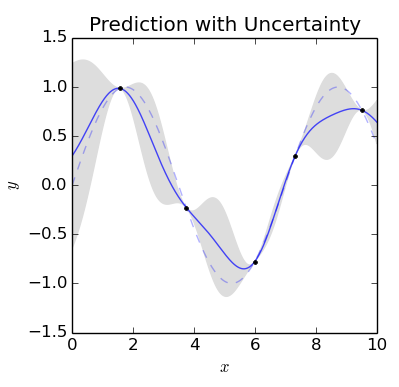
\includegraphics[width=0.4\linewidth]{Gaussian_Process_Regression.png}
	\caption{An illustration of a one-dimensional GP. The
		function used to generate the data points 
		is shown with the dashed line. The available data points are shown in
		black. The mean interpolated prediction is shown in blue
		along with the gray region showing the 68\% 
		credible interval. This figure is taken from Cdipaolo96 at 
		the Wikimedia Commons under the Creative Commons license 4.0
\label{fig:one_d_gaussian_process}}
\end{figure}


This shows the probabilistic nature of the GP predictions.
(See Fig. \ref{fig:one_d_gaussian_process})
Each drawn function represents one realization of the smoothed
field, which can be used to model the lensing potential $\psi$ later on. 
By drawing many realizations of $\psi$, we can obtain the
corresponding credible levels.
Note that the credible levels are wider for regions with less data to reflect
higher uncertainty. A GP is said to have indefinite dimension due to its ability to
predict values in unobserved regions, even though the 
observed part of the kernel is of finite size (e.g. $\ngal \times \ngal$). 
By averaging the drawn realizations, we can
obtain the mean prediction. The mean predictions from a GP are
often more well behaved and do not show drastic increase or decrease 
in the tail regions where there is no data as other polynomial interpolation schemes 
would.  

% \caption{A figure denoting a GP. The gray region represents the possible
% realizations of the GP while the red curve represents the mean prediction. 
% The width of the credible regions reflects how uncertain the predictions are,
% the less data constraints we have, the larger the uncertainty. 
% }
When the input data is mean-subtracted, we can use a zero mean function in the
GP and the covariance kernel completely specifies the GP. 
There are several families of commonly used covariance kernel.
The ones that are of the highest interest are kernels that can capture 
the homogeneity and the isotropy of the data, so the predicted spatial fields
$\psi$ can have consistent properties as the large-scale matter distribution.
On the other hand, there are other types of periodic kernels that may be useful
in modeling systematics such as masking or footprints of chip gaps due to the
stacking of multiple exposures.
For spatial models with undetermined periodicity or patterns, 
composite kernels with different covariance structures 
are formed by the addition and/or multiplication of
 to pick up (sometimes non-obvious) patterns in the data. 
A GP with composite kernels is a
famous example how both the short-and-long term trends of global carbon
dioxide level can be modeled and predicted \citep{Duvenaud2013}.

A statistical model that makes use of the GP usually decomposes 
the signal and the noise in the following way: 
\begin{equation}
	e_{\rm obs} = g + e_{}  
\end{equation}




\subsection{Adapting the exponential squared kernel with lensing physics}
One of the most popular kernels that can generate homogeneous and
isotropic data is the exponential squared kernel: 
\begin{equation}
	\kerngp(r^2) = \lambda^{-1} \exp\left(\frac{-r^2}{2 l^2}\right),
	\label{eq:exp_sq_kernel}
\end{equation}
where 
\begin{equation}
	r^2 \equiv (\xv - \yv)^T \Matrix{D} (\xv - \yv), 
\end{equation}
This kernel only depends on the
squared magnitude of distances between pairs of galaxy locations. 
This chosen form is therefore invariant
under translational and rotational transformations.
The metric $\Matrix{D}$ is taken to be a diagonal matrix but  
can be generalized to account for anamorphic distortions. 
The precision parameter $\lambda$ affects the 
amplitude of the density perturbation, while the correlation length $l^2$ 
determines how fast the correlations between different spatial locations of the
field $\psi$ fall off as a function of the spatial distance.

Additionally, the exponential squared kernel is infinitely differentiable. This
differentiable kernel choice allows us to derive an analytical expression to
relate the different lensing observables.  
In the Newtonian limit, the scalar lensing potential $\psi$ is related to 
each of the lensing observables mentioned in chapter 1, e.g. $\lensparams \equiv [\kappa, \gamma_1,
\gamma_2]$, via the following derivatives:
\begin{align}
\kappa &= \frac{1}{2}\left(\frac{\partial^2 \psi}{\partial x_1^2} +
\frac{\partial^2 \psi}{\partial x_2^2 }\right) 
= \frac{1}{2} (\psi_{,11} + \psi_{,22}),\\ 
\gamma_1 
&=\frac{1}{2}\left(\frac{\partial^2 \psi}{\partial x_1^2} - 
\frac{\partial^2 \psi}{\partial x_2^2}\right) 
= \frac{1}{2} (\psi_{,11} - \psi_{,22}), \\
\gamma_2 
&=\frac{1}{2}\left(\frac{\partial^2 \psi}{\partial x_1 \partial
x_2} + \frac{\partial^2 \psi}{\partial x_2 \partial x_1}\right)
= \frac{1}{2} (\psi_{,12} + \psi_{,21}), 
\end{align}
where we have defined the shorthand for spatial derivatives with
subscripts for $h,i,j,k = 1, 2$ after a comma.
Since the covariance operator is linear,
the derivatives for the covariance kernels of interests $\kerngp_{\rm GP}$
can be shown to be:
\begin{align}
	\label{eq:kernel_derivatives1}
	\Cov (\kappa(\xv), \kappa(\yv))
&= \frac{1}{4}\left(
\kerngp_{,1111} + \kerngp_{,1122} + \kerngp_{,2211} + \kerngp_{,2222}
\right), \\
\Cov(\kappa(\xv), \gamma_1(\yv)) &= \frac{1}{4}\left(
\kerngp_{,1111} + \kerngp_{,2211} - \kerngp_{,1122} - \kerngp_{,2222}
\right), \\
\Cov(\kappa(\xv), \gamma_2(\yv)) &= \frac{1}{4}\left(
\kerngp_{,1112} + \kerngp_{,2212} + \kerngp_{,1121} + \kerngp_{,2221}
\right),\\
\Cov(\gamma_1(\xv), \gamma_1(\yv)) &= \frac{1}{4}\left(
\kerngp_{,1111} - \kerngp_{,1122} - \kerngp_{,2211} + \kerngp_{,2222}
\right), \\
\Cov(\gamma_1(\xv), \gamma_2(\yv)) &= \frac{1}{4}\left(
\kerngp_{,1112} + \kerngp_{,1121} - \kerngp_{,2212} - \kerngp_{,2221}
\right), \\
\Cov(\gamma_2(\xv), \gamma_2(\yv)) &= \frac{1}{4}\left(
\kerngp_{,1212} + \kerngp_{,1221} + \kerngp_{,2112} + \kerngp_{,2121}
\right),
	\label{eq:kernel_derivatives2}
\end{align}
where
\begin{equation}
	\kerngp_{,hijk} = \frac{\partial^4 \kerngp}{\partial x_h \partial x_i
	\partial y_j \partial y_k}.
\end{equation}

With the definition of ${\bf \chi}_i$ as follows:
\begin{equation}
	\frac{\partial \Matrix{S}^2}{\partial \xv_i} = -\frac{\partial
	\Matrix{S}^2}{\partial \yv_i} =
	2 \Matrix{D}(\xv - \yv)_i \equiv 2{\bf \chi}_i,
\end{equation}
we can show that each entry $\nu_{,hijk}$ of $\kerngp_{,hijk}$ is
related to each entry $\nu$ of the original exponential squared kernel
$\kerngp$ by:
\begin{equation}
\nu_{,x_h x_i y_j y_k} = (\beta^4 \chi_h \chi_i \chi_j \chi_k -
\beta^3 (\chi_h \chi_i \Matrix{D}_{jk} \delta_{jk} + 5~{\rm perm.}) + \beta^2
(\Matrix{D}_{hj} \Matrix{D}_{ik}\delta_{hj}\delta_{ik} + 2~{\rm perm.})) \nu,
\label{eq:4thderivatives}
\end{equation}
with $\beta = l^{-2}$. There are 6 permutations (abbreviated as perm.) of the terms in
eq. \ref{eq:4thderivatives}
multiplied to $\beta^3$ due
to choosing two pairs of indices from the $h,i,j,k$ where the order of each
pair of indices matters when we differentiate the terms by parts. 
Likewise, there are 3 possible permutations of
the terms the multiplied to $\beta^2$ due to choosing two pairs of indices from
$h, i, j, k$ where the order of the pairs does not matter.
The derivation of the relevant derivatives and terms are available 
in the appendix for completeness. 
Our implementation of the GP kernels in eqn \ref{eq:kernel_derivatives1} - 
\ref{eq:kernel_derivatives2} is openly available at
\href{https://github.com/karenyyng/george}{https://github.com/karenyyng/george}.


\subsection{Probability framework for inferring cosmic shear}
\begin{figure}
	\centering
	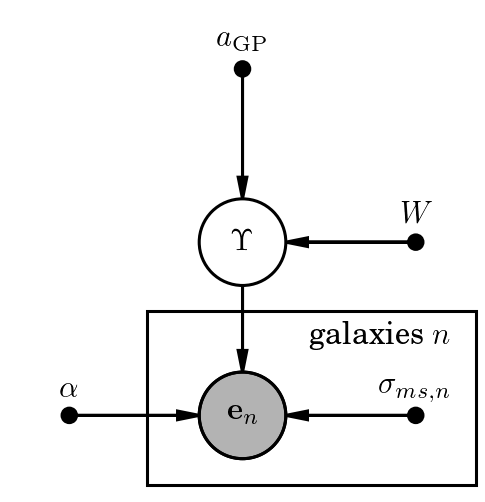
\includegraphics[width=0.4\linewidth]{shear_gp_pgm.png}
	\caption{A simplified probabilistic graphical model (pgm) for inferring
		lensing observables from survey or simulation data.
		\label{fig:simplified_pgm}}
\end{figure}






\section{Results}



\subsection{Modeling cosmic shear with the GP}
Throughout the analyses present in this work, 
we make use of the weak shear approximation 
$g = \gamma / (1 - \kappa)  \approx \gamma$, so the observed ellipticity can be
written as: 
\begin{equation}
	\epsilon_{\rm obs} = \epsilon_{\rm int} + g 
\end{equation}
assume that the shape noise term $\epsilon_{\rm int}$ of each galaxy is 
independent and follow the same Gaussian distribution.  



 
\begin{table}%[htb]
% \small
\begin{center}
\caption{Parameters for the statistical model.}
\label{tab:sampling_parameters}
\begin{tabular}{cl}
\hline
Parameter & Description \\
\hline
${\bf d_{n}}$ & data vector (measured $e_{1,2}$ for each galaxy $n$)  \\
$\sigma_{{\rm ms}; n}$ & ellipticity measurement error for galaxy $n$ 
\\
$\xv$, $\yv$ & vector(s) of 2D spatial locations of galaxies \\
$\epsilon_n^{\rm int}$ & intrinsic galaxy ellipticity for galaxy $n$ \\
$\alpha\equiv\sigma_{e}^2$ & parameters of the distribution of galaxy parameters \\
W & window function for the survey footprint \\
$\lensparams$ & lensing shear and convergence ($\gamma_{1,2}, \kappa$) \\
$\gpparams$ & parameters of the GP kernel\\
% $\rho_{\rm GP}$ & correlation of the GP kernel (element of $\gpparams$) \\
$\lambda$ & precision of the GP kernel (element of $\gpparams$) \\
$l^2$ & squared GP correlation length (element of $\gpparams$) \\
% $\lambda_{\epsilon}$ & precision for the nugget term (element of $\gpparams$) \\
\hline
\end{tabular}
\end{center}
\end{table}



\subsection{Verification using {\sc GalSim} simulated data}
\subsection{Mass mapping for Deep Lens Survey Abell 781}

% Is a non-trivial optimization problem 

\section{Discussion}

\subsection{Relating the lensing observables to a cosmological model}


We can draw realizations of the lensing observables from the GP given a set of
optimized GP parameters:
\begin{equation}
	\lensparams(\xv) \sim GP(0, \kerngp_{\rm GP}(\xv, \yv)) 
\end{equation}


The constraints on cosmological parameters need to be verified in a mock
weak-lensing analysis of cosmological simulation. 
It can enable the separation of E and B mode in the convergence field as shown
in Schneider et al. (in prep.) 

\subsection{Use of the Gaussian Process in the model fitting for shear}
We describe a simplified graphical model to demonstrate how the derived GP can
be used to infer cosmic shear and a mass map from the convergence.
A more sophisticated model can be found in Schneider et al. 2016.



% - [ ] TODO add PGM 
% talk about the lensing approximations that were made 


% \subsection{Sampling grid and the correlation length}
% A weakness of the method is the apparent reliance on having the sampling 



\subsection{Separation of the E / B mode}
Under the same formalism, it is also possible to rewrite our covariance kernel 
to separate the E and the B mode of the shear, those derivation can be seen in  
\cite{Schneider2001a}.

\begin{align}
	\kappa^E & = \kappa\\
	\kappa^B & = 0 \\
	\gamma^E &= \left[\frac{1}{2} (\psi^E_{,11} - \psi^E_{,22}) -
	\psi^B_{,12}\right]\\
	\gamma^B &= \left[\psi^E_{,12} + \frac{1}{2} (\psi^E_{,11} - \psi^B_{,22})\right]
\end{align}


\subsection{Modeling systematics and noise}
% Can handle sharp boundaries from stacking images 
% cite Jee2013a  
% cite Rowe2010 paper for interpolating star fields for 
% PSF ellipticity corrections 

\subsection{Alternative kernel choice(s) for encoding the lensing physics}
Alternative choices for a covariance kernel for describing the lensing physics 
include the family of Mat\'{e}rn kernels.
[TODO add form of expression] 
The smoothness of the data generated from a Mat\'{e}rn kernel is closely
related to the degree of freedom of the kernel. 
The higher degree of freedom it has, the smoother the spatial variations of the
drawn $\psi$ would be for the same correlation length.
Note that a Mat\'{e}rn kernel is also only differentiable to the $i$-th order,
where $i$ is [TODO] related to the degree of freedom by [TODO].
This restricts us to use kernels with degree of freedom above [TODO]. 
When we take the limit of the degree of freedom of a Mat\'{e}rn kernel to infinity, 
we recover the exponential squared kernel.

It is possible to generalize the derivation of derivatives by using automatic
differentiation. Automatic differentiation may allow evaluation of other
kernels that generates isotropic and homogeneous data, 
such as the Mat\'{e}rn kernels.  
% An implementation via numerical differentiation may
% or may not be more computationally intensive to
% compute, depending on the required numerical precision (aka order of accuracy).
Differentiation technology such as automatic differentiation, 
that spreads factors of the derivatives over a tree like structure for
almost exact computation can be considered, but is outside the scope of this work.

\subsection{Computational performance of our method}
We implemented the covariance kernels in \ref{eq:kernel_derivatives1}
via {\sc C++} along with a {\sc Python} wrapper. 
Although the operation of computing and assembling the
derivatives are $O(\ngal^2)$, the large number of addition and 
multiplication operations can be slow.
Exploiting the symmetry of the covariance kernel can only provide 
memory saving of a factor of 2.
The parallelized computation of each element of the kernel was achieved using 
the {\sc OpenMP} library. The slowest step of the entire computation, however, 
is the inversion of the
covariance kernel matrix for the evaluation of the marginal likelihood, 
which is a $O(\ngal^3)$ operation. 
We made use of parallelized Cholesky decomposition via the {\sc Intel Math
Kernel Library}
to perform the inversion of the matrix and achieved $\sim10$ times speed up so the
computation and the evaluation of the likelihood of each set of GP parameter
take $< 10s$ for 1000 galaxies, which translates to a 3000 $\times$ 3000
covariance matrix.
Currently, our method is not computationally competitive as the 2PCF, those
fastest distributed and parallelized 
implementation has a computational complexity of $O(N\sqrt{N})$ \citep{Chhugani2012}.

Rather than relying on manual intensive methods for parallelizing the
computation of the kernel methods, a more promising way is to approximate the
small elements in the covariance kernel structure as zero. 


With large amount of
sparsity, The inversion of the matrix can be sped up to [TODO]$O(M^2N)$ for
building the model and $O(M^2)$ for interpolating / predicting output functions
at new input locations \citep{Snelson2006}.
The relevant field of literature about how the approximations may affect the
statistical inference is called covariance tapering. On the other hand,  
the Machine Learning community refer to the support for the approximate kernel
as induce point methods.

  

\section{Conclusion}
Here, we have derived and implemented a fully probabilistic method for 
representing the lensing observables. It can potentially  

The potential of using a Gaussian Process for the inference of cosmological 
Gaussian Process (GP)parameters remains to be proved. 

\section{Acknowledgement}
We thank Chris Paciorek for discussion about the statistical
framework for performing shear inference and the
use of Gaussian Processes.
This research
used the resources of the National Energy Research Scientific 
Computing Center (NERSC), a DOE Office of Science
User Facility supported by 
of the U.S. Department of Energy under Contract No.
DE-AC02-05CH11231.
 This work uses a modified version
of the public code {\sc George} available at \href{https://
github.com/karenyyng/george}{https://
github.com/karenyyng/george}, which was forked from \\
\href{https://github.com/dfm/george}{https://github.com/dfm/george}.



\appendix 

\section{Derivation of GP kernel}

\begin{equation*}
\Sigma = \lambda^{-1} \kerngp 
\end{equation*}

\begin{align}
\kerngp &= \exp{\left(\frac{-\beta}{2} r^2 \right)}\\
\kerngp_{,x_i} &= \frac{-\beta}{2} k r^2_{,x_i} = -\beta \kerngp X_i\\ 
\kerngp_{,y_h} &= \beta \kerngp X_h 
\end{align}

\begin{align}
\kerngp_{,x_i x_j} &= \frac{-\beta}{2}(\kerngp_{,x_j} r^2_{,x_i} + 
\kerngp r^2_{,x_i x_j})\\
\kerngp_{,x_i x_j y_h} &= \frac{-\beta}{2}(\kerngp_{,x_j y_h} r^2_{,x_i} + \kerngp_{,x_j}
r^2_{,x_i y_h} + \kerngp_{,y_h} r^2_{,x_i x_j})\\
\kerngp_{,x_i x_j y_h y_k} &= \frac{-\beta}{2} 
(\kerngp_{,x_j y_h y_k} r^2_{,x_i} +
\kerngp_{,x_j y_h} r^2_{,x_i y_k} + 
\kerngp_{,x_j y_k} r^2_{,x_i y_h} + 
\kerngp_{,y_h y_k} r^2_{,x_i x_j} )
\end{align}

Just work on terms that are parts of the 4th kernel derivative 
\begin{align*}
\kerngp_{,x_i x_j} &= \frac{\partial}{\partial x_j} (-\beta \kerngp X_i)\\
&= -\beta(\kerngp_{,x_j X_i} + k X_{i, x_j})\\ 
&= -\beta(-\beta \kerngp X_j X_i + \kerngp \delta_{ij} D_{ij}) \\ 
&= (\beta^2 X_j X_i - \beta \delta_{ij} D_{ij})\kerngp 
\end{align*}

\begin{align*}
\kerngp_{,x_i y_h} &= \frac{\partial}{\partial y_h} (-\beta \kerngp X_i)\\
&= -\beta(\kerngp_{,y_h X_i} + \kerngp X_{i, y_h})\\ 
&= -\beta(\beta \kerngp X_h X_i - \kerngp \delta_{ih} D_{ih}) \\ 
&= -(\beta^2 X_h X_i - \beta \delta_{ih} D_{ih})  
\end{align*}

\begin{align*}
\kerngp_{,y_h y_k} &= \frac{\partial}{\partial y_h} (\beta k X_h)\\
&= \beta(\kerngp_{,y_k X_h} + k X_{h, y_k})\\ 
&= \beta(\beta k X_k X_h - k \delta_{hk} D_{hk}) \\ 
&= (\beta^2 X_h X_k - \beta \delta_{hk} D_{hk})\kerngp 
\end{align*}

\begin{align}
\kerngp_{,x_i x_j} &= (\beta^2 X_j X_i - \beta \delta_{ij} D_{ij})\kerngp\\ 
\kerngp_{,x_i y_h} &= -(\beta^2 X_h X_i - \beta \delta_{ih} D_{ih})\kerngp\\ 
\kerngp_{,y_h y_k} &= (\beta^2 X_h X_k - \beta \delta_{hk} D_{hk})\kerngp 
\end{align}

\subsection{Term 1 of the 4th derivative of eqn [TODO]}
\begin{align*}
\kerngp_{,x_j y_h y_k}
&= \frac{\partial}{\partial y_k} \kerngp_{,x_j y_h}\\ 
&= -\frac{\partial}{\partial y_k} (\beta^2 X_h X_j - \beta \delta_{jh} D_{jh})\kerngp\\
&= (\beta^2 D_{hk} \delta_{hk} X_j + \beta^2 X_h D_{jk}\delta_{jk})\kerngp -
(\beta^2 X_h X_j - \beta D_{jh} \delta_{jh})\beta X_k k
\end{align*}

\begin{align*}
&\kerngp_{,x_j y_h y_k} r_{,x_i}^2\\
&= 2[\beta^2 X_j D_{hk} \delta_{hk} + \beta^2 X_h D_{jk}\delta_{jk} +
\beta^2 X_k D_{jh} \delta_{jh} - \beta^3 X_h X_j X_k] X_i k\\ 
&=\boxed{2\beta^2[ 
X_j X_i D_{hk} \delta_{hk} + 
X_h X_i D_{jk} \delta_{jk} + 
X_k X_i D_{jh} \delta_{jh}] k  
- 2\beta^3 X_h X_j X_k X_i k} 
\end{align*}

\subsection{Term 2 of the 4th derivative}
\begin{align*}
\kerngp_{,x_j y_h} r^2_{,x_i y_k}
&= - (\beta^2 X_h X_j - \beta D_{jh} \delta_{jh}) (-2D_{ik} \delta_{ik}k) \\  
&= \boxed{( 2 \beta^2  X_h X_j D_{ik} \delta_{ik} 
-2 \beta D_{jh} D_{ik} \delta_{jh} \delta_{ik}) k} 
\end{align*}

\subsection{Term 3 of the 4th derivative}
This is completely analogous to term 2 except the subscripts are slightly
different
\begin{align*}
\kerngp_{,x_j y_k} r^2_{,x_i y_h}
&=\boxed { ( 2 \beta^2  X_k X_j D_{ih} \delta_{ih} 
-2 \beta D_{jk} D_{ih} \delta_{jk} \delta_{ih}) \kerngp} 
\end{align*}

\subsection{Term 4 of the 4th derivative} 
\begin{align*}
\kerngp_{,y_h y_k} r^2_{,x_i x_j}
&= (\beta^2 X_k X_h - \beta D_{hk}\delta_{hk})\kerngp 2 D_{ij} \delta_{ij}\\ 
&= \boxed{(2\beta^2 X_k X_h D_{ij} \delta_{ij} - 2\beta D_{ij} D_{hk} \delta_{hk}
\delta_{ij})\kerngp } 
\end{align*}

Collect terms of $\Sigma_{,x_i x_j y_h y_k}$ by plugging them in eqn 20 
All the relevant terms are boxed above, 
\begin{align}
\nu_{,x_i x_j y_h y_k} &= (\beta^4 X_h X_j X_k X_i -  
\beta^3 (X_j X_i D_{hk} \delta_{hk} + 5 {\rm perm.}) + \beta^2
(D_{jh} D_{ik}\delta_{jh}\delta_{ik} + 2 {\rm perm.})) \nu \\
&= \gamma \nu
\end{align}

Where $\nu$ is an entry in the matrix $\Sigma$
\begin{equation}
\Sigma  = 
\left(
\begin{array}{ccc}
\nu_{11} & \cdots & \nu_{1n} \\
\vdots & \ddots & \vdots \\
\nu_{n1} & \cdots & \nu_{nn} \\
\end{array}
\right)
\end{equation}


